\documentclass[]{article}

\begin{document}
\section{Keuze programmeertaal: Java}
We hebben gekozen voor Java omwille van het grote aanbod van uitgebreide API's. Beide teamleden zijn bekend met de programmeertaal door de cursus object-geori\"{e}nteerd programmeren 2. \\\\
Ook is de taal cross-platform wat een eis is van het project. Andere talen zoals C++ kunnen ook cross-platform applicaties maken, echter is Java meer out-of-the-box cross-platform. Tenzij de programmeur speciale libaries zou gebruiken, is de applicatie altijd cross-platform.\\\\ Multithreaded programmeren wordt ook versimpeld door gebruik te maken van de \texttt{Thread} libary die Java aanbiedt. Hiermee kan de uitvoering op een andere thread gebeuren dan de uitvoering van de GUI. \\\\De automatische garbage collection van Java zorgt er voor dat er snel een werkende applicatie kan gerealiseerd worden.  Java biedt ook een sterke GUI libary aan nl.  \texttt{Swing}. 

\section{Views-Models-Uitvoering}
Het programma is opgebouwd uit drie grote modules. Deze keuze werd gemaakt om de ontwikkeling op te kunnen splitsen. Zo werd eerst de  uitvoerings module gebouwd zodat er zekerheid was over de werking van de applicatie. Hoewel de creatie van een programma om deze manier omslachtig is, kon deze module grondig getest worden.\\\\
Na een cree\"{e}ren van een betrouwbare uitvoering, kon de Model module worden uitgewerkt. Hierin werd de applicatie logica gestoken. Na het vervolledige van deze module werd de connectie gemaakt tussen de uitvoering en de model module. Dit in vorm van een compiler.\\\\
Door het inladen en opslaan van een programma mogelijk te maken via de model module kan er snel een programma worden geschreven in het gekozen bestandsformaat (XML). Het opslaan en inladen gebeurt via interfaces, het gebruikte opslagformaat kan dus ook simpel aangepast worden door andere implementerende classes te maken. \\\\
Daarna is de Views module opgebouwd. Doormiddel van de implementatie van de DataEditor kon gemakkelijk de correctheid van een programma gecontrolleerd worden. Dit door de reeds betrouwbare backend.\\\\
De opbouw van het programma om deze manier brengt een aantal extra voordelen mee. Zo staat de backend (de uitvoering), de model logica en de view apart van elkaar. Door andere executieblokken en een andere compiler te schrijven kan een programmeur zeer eenvoudig een nieuwe backend voorzien. De koppeling tussen de drie modules gebeurt door basis klassen zoals BlockModel, of de Compiler klasse. De frontend kan ook volledig aangepast worden losstaand van de executie. 
\subsection{Pipeline}
In onderstaande figuur word de volledige pipeline getoond van een enkele blok. Er kan gezien worden dat de views enkel communiceren met de models. Deze models zitten in de ModelCollection die in verbinding staat met de runtime en de compiler. De runtime (en de compiler) vormt de verbinding tussen de models en de uitvoerblokken. Er is te zien dat er verder geen verbindingen zijn tussen de models en de uitvoer. In de volgende secties zullen de verschillende componenten van deze pipeline in detail besproken worden.
 \begin{sidewaysfigure}[h]
  \centering
   
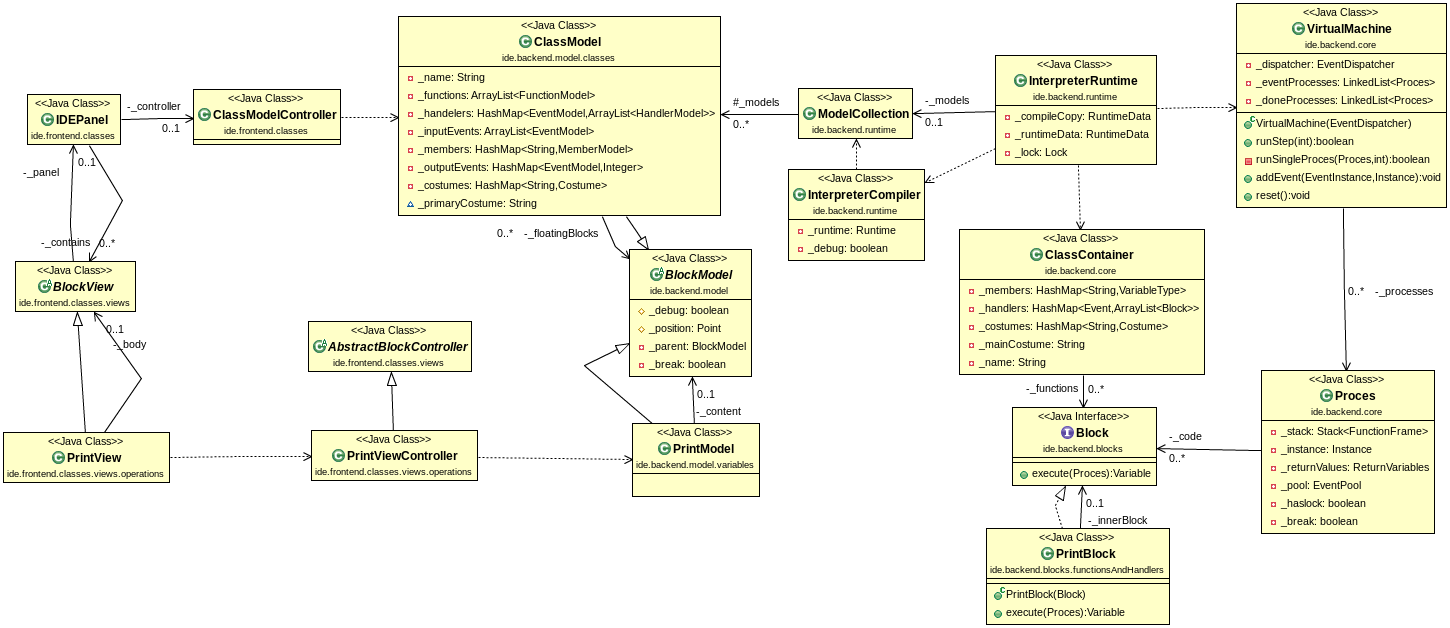
\includegraphics[scale=0.4]{./AnalyseADTAlgorithm/pipelinePrintBlock.png}
  \caption{Pipeline.} \label{gui}
\end{sidewaysfigure}
\clearpage


\section{Modellen}
\label{Modellen}
\subsection{Nesting van blokken}
Een programma opgebouwd uit blokken kan gezien worden als een boom. Hierbij vormen de verschillende functies of handlers verschillende deelbomen en stellen blokken bladeren voor in deze deelbomen. Om logica in het nesten van blokken te steken is er nood aan onderlinge communicatie tussen de blokken. Zo moet een blok informatie aan zijn kinderen kunnen geven en een kind informatie aan zijn ouder.\\\\
Een kind moet ook zijn boom kunnen afsporen om te kijken van welke deelboom hij deel uitmaakt. Een voorbeeld hiervan in een return block. Deze zal nagaan als hij tot de deelboom van een functie behoort en wat het return type is van de functie.\\\\
Ook is er nood om de applicatie logica te scheiden van het visuele gedeelte van het programma. Hierdoor kan het visuele gedeelte makkelijk veranderd worden zonder dat de logica verloren gaat.\\\\
De volgende sectie bespreekt hoe beide deelproblemen worden opgelost in de implementatie doormiddel van het invoeren van Modellen.
\subsection{Modellen, Visuele representatie en Controller}
De applicatie logica voor het opbouwen van een progamma wordt gescheiden van 
visualisatie van een programma door door de invoering van  het concept Model. Dit model beheert de applicatie logica van de blok. Een visuele block (view) kan dan communiceren met zijn model via een controller. En zal veranderingen aan het model observeren door middel van het Oberver Pattern \cite{Observer_pattern}. Het patroon wat beschreven wordt doormiddel van deze drie componenten: Model, View en Controller is het MVC patroon.

\subsection{Implementatie}
Deze sectie zal de implementatie in het programma bespreken van bovenstaande concepten en deelproblemen. Eerst worden de twee basis modellen \textbf{BlockModel} en  \textbf{ConnectedBlocks} besproken.  BlockModel stelt een knoop voor in de boom van blokken. ConnectedBlocks wordt gebruikt voor een collectie knopen met dezelfde ouder.\\\\
\textbf{Onderlinge Communicatie} bespreekt hoe de onderlinge communicatie tussen ouder en kind werd ge\"{i}mplementeerd. Hierna volgen enkel specifi\"{e}ke modellen van blokken die van deze communicatie gebruik maken besproken. Dit zijn opeenvolgend \textbf{Variabelen}, gedrag van een  \textbf{Access blok in een Handler}, gedrag van een \textbf{Return blok} en het gedrag een \textbf{Emit blok}. Ook de implementatie van \textbf{TypeChecking}  wordt besproken.

\subsubsection{BlockModel}
\label{BlockModel}
BlockModel is de basis klasse voor het model van elke block. sBlockModel leidt af van de abstracte klasse \texttt{java.util.Observable} \cite{Observable}. Een BlockModel bevat de volgende basis attributen: Een Blockmodel parent, een positie, een debug status en een break status. De parent attribut verwijst naar de block waarin de block zich bevindt. Voor een top level block zoals een functie of handler zal dit \texttt{null} zijn. Ook voor blokken die nergens toe behoren zal dit zo zijn.\\\\
De positie van de block wordt opgeslaan voor het inladen van een programma mogelijk te maken. Deze zal dus geupdate worden bij elke verplaatsing.\\\\
De attributen debug status en break worden in detail besproken in Sectie~\ref{Debug}.
\subsubsection{ConnectedBlocks}
\label{connectedBlocks}
Naast het inelkaar steken van blokken is er ook de nood om blokken onderelkaar te plaasten of meerder blokken in eenzelfde block te steken. Zoals bijvoorbeeld de body van een if-statement. Hiervoor wordt de de klasse ConnectedBlocks gebruikt. Deze is afgeleid van een BlockModel en bevat dus dezelfde functionaliteit. Alle blokken die zich in een ConnectedBlocks bevinden zullen dezelfde parent hebben namelijk die connectedBlock. Bij het verwijderen van een blok uit de connectedBlock zal een nieuwe connectedBlock worden gecree\"{e}rd. Deze bevat de verwijderde blok plus alle blokken die zich onder deze blok bevonden. 
\subsubsection{Onderlinge Communicatie}
\label{onderlingeCommunicatie}
Om de applicatie logica te implementeren was er nood aan een onderlinge communicatie tussen blokken. Een parent-blok moet zijn kind kunnen verwittigen voor veranderingen maar ook communicatie in de andere richting is gewenst.\\\
Deze communicatie wordt mogelijk gemaakt door volgende functies uit BlockModel \texttt{changeParent} en \texttt{tellParentChanged}. Doormiddel van \texttt{changeParent} laat een parent weten aan zijn kind(eren) dat deze veranderd is naar de meegeven BlockModel. \texttt{tellParentChanged} geeft de mogelijkheid om een kind te laten weten wat zijn type is en wie hij is (mogelijks heeft een parent meerdere kinderen).
\begin{figure}[H]
  \centering
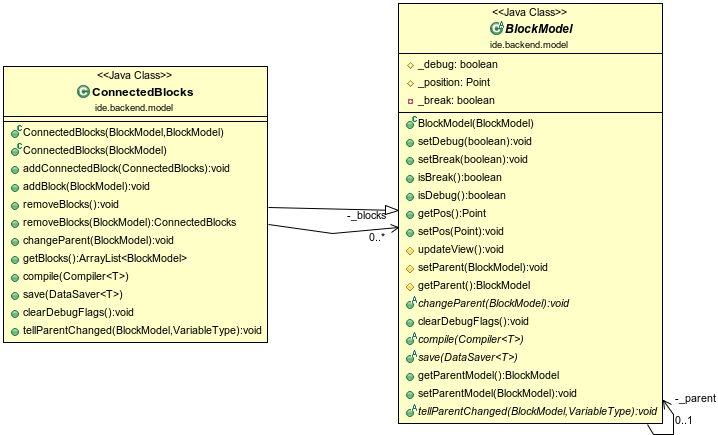
\includegraphics[scale=0.4]{AnalyseADTAlgorithm/blockmodel/baseclassuml}
  \caption{BlockModel en ConnectedBlocks.} \label{BlockModelUML}
\end{figure}

\subsubsection{Variabelen}
\label{variabelen}
Bij variabelen wordt er een onderscheidt gemaakt tussen lokale variable en membervariabelen van een klasse. Voor hun gemeenschappelijke basis en eenvoud in gebruik op plaatsen waar geen onderscheid moeten worden gemaakt worden zowel voor de declaratie modellen als referentie modellen een abstract basis klasse ingevoerd. Dit zijn respectievelijk AbstractVariableModel en AbstractRefVariabelModel (Figuur~\ref{varModelUML}). \\\\
\begin{figure}[H]
  \centering
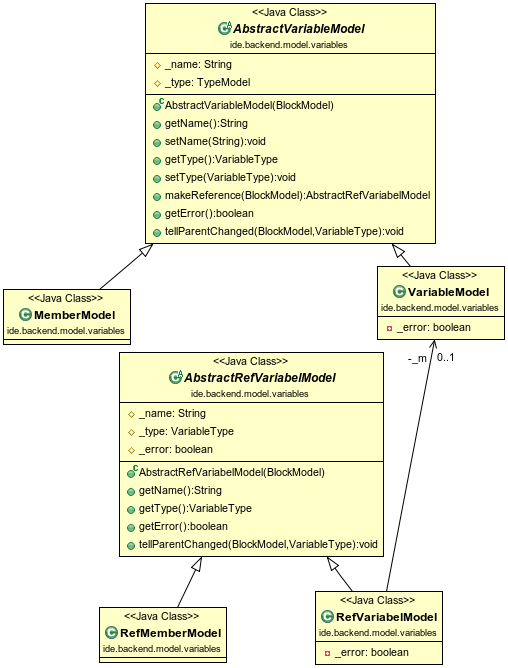
\includegraphics[scale=0.4]{AnalyseADTAlgorithm/blockmodel/variablemodels}
  \caption{VariableModels} \label{varModelUML}
\end{figure}
Variabelen zijn een voorbeeld waarbij er nood is aan onderlingen communicatie tussen parent en child. Een declaratie van een lokale variabele gebeurt door een VariableModel. Een lokale variabele bestaat enkel in de scope van een een Handeler of Functie. TopLevel blok is een abstracte basis klasse die afleid van BlockModel voor een functie of handler. Deze Klasse houdt een lijst bij van alle namen van zijn lokale variabele.\\\\
\begin{figure}[H]
  \centering
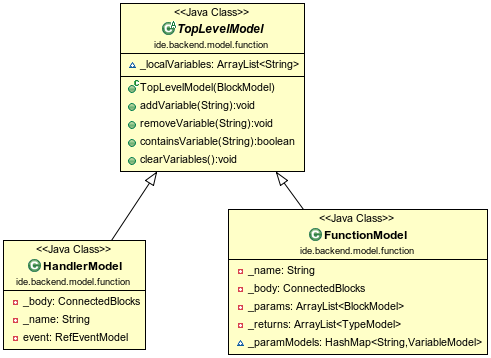
\includegraphics[scale=0.4]{AnalyseADTAlgorithm/blockmodel/topleveluml}
  \caption{TopLevelModel} \label{TopModelUML}
\end{figure}
Bij het toevoegen van een VariableModel aan een TopLevelModel zal deze al zijn kinderen laten weten dat hun parent veranderd is. Dit wordt doorgegeven tot onderste kinderen (een variable is altijd het einde van een tak).\\\ Als op een VariableModel de \texttt{changeParent} functie wordt opgeroepen zal deze nakijken als hij zich bevindt in een ToplevelBlock, dit doormiddel van onderstaande pseudo code. Zoja, als deze veranderd is, wordt er gevraagd als de naam van de variabele al in gebruik is. Zoja, wordt een error getoond aan de gebruiker (Figuur~\ref{errorvars}). Anders, wordt deze toegevoegd. Er moet ook bij verandering van naam hiermee rekening worden gehouden.  Bij het verwijderen zal de variabele uit de lijst moeten worden verwijderd.\\\\
\lstset{language=Java}
\begin{lstlisting}
Zoek functie of handler waartoe blok behoort(){
		als heeft Parent{
			huidig = getParent();
			Zolang handler of functie niet gevonden en niet top van boom bereikt{
				loop naar boven in boom en houdt positie bij huidig.
			}
		}
		Als huidig een functie of handler is
			geef huidig terug.
		anders
			geef null terug.
			
	}
\end{lstlisting}
Referenties naar een lokale variabele moeten ook in dezelfde scope zitten als hun declaratie. Dit moet duidelijk gemaakt worden aan de gebruiker. Dit wordt gerealiseerd op dezelfde manier. Een RefVariableModel zal bij oproep van \texttt{changeParent} zoeken naar zijn TopLevelModel. Deze vergelijkt hij met het TopLevelModel van de VariableModel naar welk hij refereert, waarvan hij een referentie bezit. Als deze niet gelijk zijn wordt er een error getoond aan de gebruiker (Figuur~\ref{errorvars}).\\\\ 
\begin{figure}[H]
  \centering
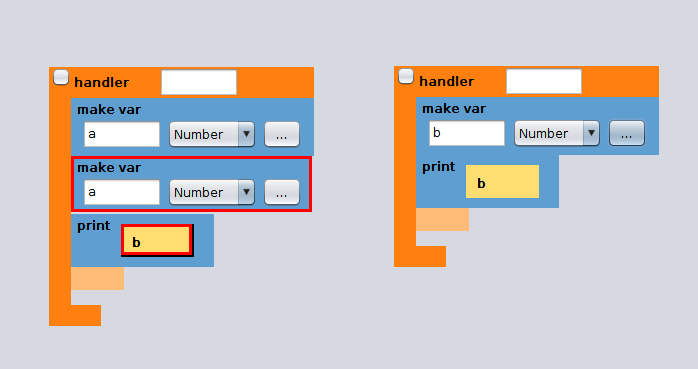
\includegraphics[scale=0.4]{AnalyseADTAlgorithm/blockmodel/errorvars}
  \caption{Error duplicate naam en foute scope.} \label{errorvars}
\end{figure}

\subsubsection{AccessModel en HandlerModel}
\label{access&Handler}
Een access blok wordt gebruikt voor informatie uit een InputEvent dat verwerkt wordt door een handler op te halen. Uiteraard moet een access blok weten als hij al dan niet in een handler steekt. Dit kan door bij het oproepen van de \texttt{changeParent} te gaan zoeken naar zijn TopLevel en na te kijken als dit een handler is. En als deze Handler reeds verbonden is met een InputEvent. Als een handler van een InputEvent wordt verwijderd of veranderd. Kan deze verandering makkelijk worden doorgegeven worden door dezelfde \texttt{changeParent} functie. Als een AccesModel zijn Event heeft gevonden kan een member geselecteerd worden. En kan het type van de member worden opgevraagd. Dit kan dan gebruikt worden voor de typechecking (Sectie~\ref{TypeChecking}).
\begin{figure}[H]
  \centering
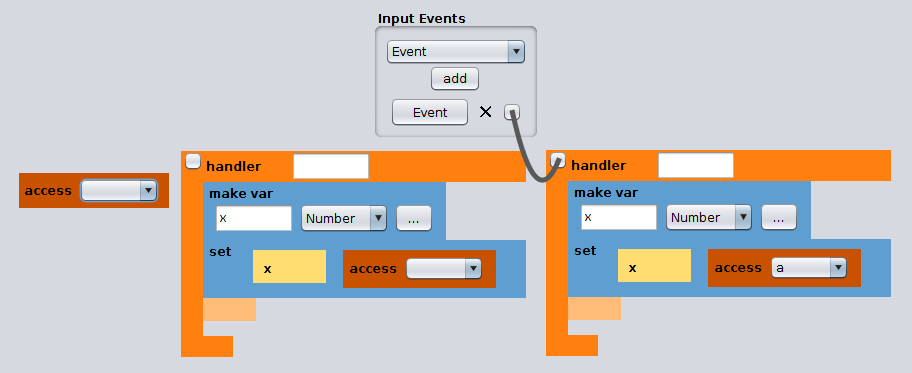
\includegraphics[scale=0.4]{AnalyseADTAlgorithm/blockmodel/accesHandler}
  \caption{Access blok zoekt naar Event handler.} \label{findhandler}
\end{figure}

\subsubsection{ReturnModel en FunctionModel}
\label{returnModel}
Een ReturnModel werkt op een gelijkaardige manier als een AccessModel. Bij het veranderen van zijn parent zal hij zoeken als hij zich in een FunctieModel bevindt. Zoja, vraagt hij naar het return type zodat hiermee type checking kan gebeuren (Sectie~\ref{TypeChecking}).

\subsubsection{EmitModel}
\label{EmitModel}
Een emit blok wordt gebruikt voor verzenden van OutputEvents. Het kan zijn dat een Event Members bevat die dan ingevuld moeten worden. Het is duidelijk dat een EmitModel moet weten welke Events er allemaal beschikbaar zijn in het programma. Deze kan hij ophalen uit de ModelCollection (Sectie~\ref{ModelCollection}). Na het selecteren van een Event kan een EmitModel net zoals een AccessModel nagaan wat de type(s) zijn van de member(s). Dit kan dan weer gebruikt worden voor type checking (Sectie~\ref{TypeChecking}). Aangezien de members van een EventModel ook VariableModels zijn, kunnen deze geobserveerd worden voor veranderingen. Bij een verandering zoals het type. Zal dit worden geupdate in het view van het model . 
  

\subsubsection{TypeChecking}
\label{TypeChecking}
Door gebruik te maken van eerder beschreven functies \texttt{changeParent} en \\ \texttt{tellParentChanged} wordt typechecking ge\"{i}mplementeerd in het programma. Uiteraard heeft niet elke blok een type en moet niet iedere blok aan zijn parent melden wat zijn type is.\\\\
Voor sommige blokken zoals SetModel is de implementatie eenvoudig. SetModel kan gebruikt worden om de waarde van twee variable of een variable en een waarde aan elkaar gelijk te stellen. Hier moet de parent nakijken na het ontvangen van het type van beide kinderen als er een error optreed (zie onderstaande code fragment).\\\\
\lstset{language=Java}
\begin{lstlisting}
public void tellParentChanged(kind , type van kind) {
		_fout = false;
		als kind is rechter kind
			_rechter type is type van kind;
		Als SetBlock volledig{
			als (types niet overeenkomen  en rechter type is geen letterijke waarde )
				_fout = true
		}
		Laat view weten dat er een fout is.
	}
\end{lstlisting}
Doordat een AbstractRefVariableModel bij verandering van type van de variabele waarnaar hij verwijst opnieuw aan zijn parent laat weten dat er een verandering is. Kan bij elke verandering een error onstaan of ongedaan gemaakt worden (Figuur~\ref{typeCheckerror}).
\begin{figure}[H]
  \centering
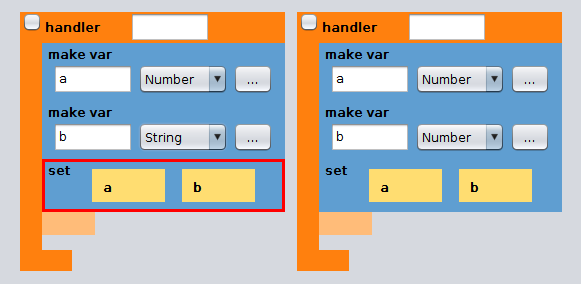
\includegraphics[scale=0.4]{AnalyseADTAlgorithm/blockmodel/typecheckError}
  \caption{Typecheck error.} \label{typeCheckerror}
\end{figure}
Type checking voor gebeurt op een gelijkaardige manier voor de volgende blokken: EmitModel, AccessModel, ReturnModel, MoveModel, CharAtModel en LengthModel.\\\\
Voor de operator blok gebeurt dit anders. Een unaire en binaire operatie worden respectievelijk voorgesteld door een UnOperatorModel en een OperatorModel.
Deze klassen maken gebruik van een TypeChecking klasse. Bij het ontvangen van de types van beide operanden zal worden nagekeken als de operatie mogelijk is en wat het return type is van de operatie. Dit return type kan dan weer verder worden doorgegeven. 

\begin{figure}[H]
  \centering
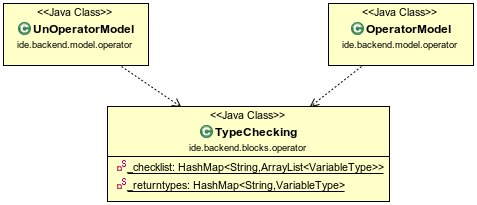
\includegraphics[scale=0.4]{AnalyseADTAlgorithm/blockmodel/operatorType}
  \caption{Operators.} \label{Operators}
\end{figure}

\subsection{ModelCollection}
\label{ModelCollection}
De data van een programma wordt bewaart in drie delen. Namelijk het WireFrameModel wat alle informatie bevat over de bestaande instanties en de connecties tussen deze instanties. De EventModels die de bestaande Events beschrijven. En de ClassModels die de bestaande klassen beschrijven. \\\\
Om interactie tussen deze modellen mogelijk te maken en alle informatie centraal te verzamelen. Wordt er een data klasse ingevoerd, de ModelCollection klasse bewaart alle informatie van het programma. Hierdoor kan ervoor gezorgd worden dat aanpassingen in een module door kunnen worden gegeven aan een andere module.\\\\
Deze data collectie wordt gebruikt om het programma te compileren, op te slaan of in te laden.
\begin{figure}[H]
  \centering
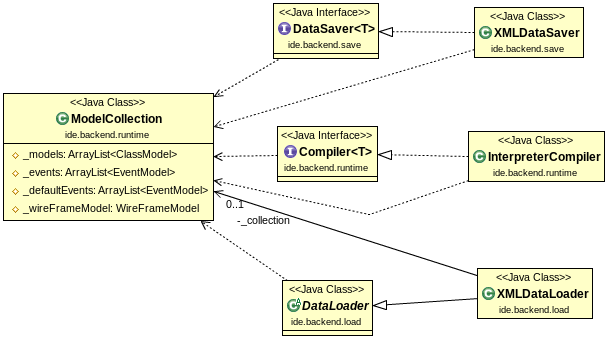
\includegraphics[scale=0.4]{AnalyseADTAlgorithm/ModelCollection/ModelCollection.png}
  \caption{ModelCollection.} \label{modelCollectionImage}
\end{figure}


\section{Executie}
\label{Algoritme}
Zoals al eerder vermeld in dit verslag is dient onze applicatie om event-driven programma's te maken. In de volgende sectie wordt er kort uitgelegd wat het \textbf{event-driven programming} paradigma inhoudt en hoe dit ge\"{i}mplementeerd werd. De uitvoer verloopt concurrent. Er is gekozen om een \textbf{eigen interpreter} te schrijven. Hierdoor is er volledige controle over de concurrente uitvoering.  \\\\
De uitvoeromgeving is opgesplitst in enkele onderdelen. De \textbf{runtime} die op hoog niveau controle heeft over het programma, zoals het laten lopen of stoppen van een programma. Events verzonden door de gebruiker moeten opgevangen worden en doorgestuurd worden naar de uitvoering. Dit gebeurt door de \textbf{EventCatcher}. Er moet een omzetting gebeuren van de bestaande modellen naar een uitvoerbaar formaat. Dit gebeurt door gebruik te maken van een \textbf{Compiler}. \\\\
De eigenlijke uitvoering moet ook geregeld worden. Het schedulen van de verschillende gesimuleerde threads moet effici\"ent en eerlijk gebeuren. Di is de taak van de \textbf{virtual machine}. Er moet ook ondersteuning geboden worden voor \textbf{debugging}. Het probleem bij de implementatie van debugging is het vermijden van het vervuilen van de gewone uitvoering. 
\subsection{Event-driven programming.}
Event-driven programming is een programmeer paradigma waarbij de flow van het programma wordt bepaald door events gecree\"{e}rd door de gebruiker zoals input events of door events veroorzaakt door delen in het programma \cite{eventdrivenwiki}.

\subsubsection{Extended handlers design pattern}
Als design pattern voor onze applicatie hebben we ons gebasseerd we op het extended handlers design pattern dat Stephen Ferg uitlegt in zijn paper: Event-Driven Programming: Introduction, Tutorial, History \cite{eventdrivenStephen}.
\begin{figure}[H]
  \centering
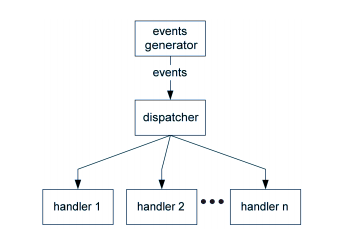
\includegraphics[scale=0.5]{AnalyseADTAlgorithm/extendedHandlerspattern.png}
  \caption{Extended handler.} \label{extendedHandler}
\end{figure}

In Figuur \ref{extendedHandler} stelt de eventgenerator in onze applicatie het generenen van events door gebruikers input en door instanties voor. Door dat events talrijk gegenereerd kunnen worden zal de Dispatcher een queue zijn die een stroom van events opvangt. Hij zal ervoor zorgen dat het event door de juiste handelers wordt afgewerkt.\\\\
Doordat in onze applicatie events worden doorgegeven aan specifieke andere instanties van Klassen zoals beschreven in de Sectie \ref{Events}. Zal de dispatcher ervoor moeten zorgen dat de juiste handlers van de juiste instanties worden aangeroepen.

\subsection{Concurrent computing }
Concurrent computing \cite{concurrent} is een vorm van computing waarbij een deel berekeningen worden uitgevoerd zodat het lijkt alsof ze gelijktijdig worden uitgevoerd. We hebben ervoor gekozen om niet multi-threaded te werken om de complexiteit van het project zo laag mogelijk te houden.\\\\ Daarom is concurrent computing de oplossing voor onze applicatie. In tegenstelling tot parallel computing is dit wel mogelijk op een thread. Gelijktijdige processen zoals twee events die samen worden opgeroepen lijken hierdoor ook gelijk te worden afgehandeld. In tegenstelling tot het sequentiel uitvoeren van de twee events.\\\\
Bij concurrent computing worden processen in executie stappen opgedeeld. Er wordt gebruik gemaakt van timeslices waarin van elk proces een deel executie stappen worden uitgevoerd, wij noemen dit een primitieve stap. Na dat bepaald aantal of tijd wordt het proces gepauzeerd en verder gegaan met het volgende. Dit wordt herhaald zolang een proces niet volledig is afgerond.
\subsubsection{Verschil met parallel computing}
Parallel computing is gelijkaardig aan concurrent computing, echter gebeurt het werk op verschillende cores. Bij concurrent computing zal de uitvoering van twee identieke events die gelijktijdig worden aangeroepen niet gelijktijdig eindigen omdat de uitvoering steeds wisselt tussen de twee events. 

\subsubsection{Probleem met concurrent computing}
Een eerste probleem is \textbf{racing conditions}. Hierbij proberen twee processen hetzelfde algortime uit te voeren waarbij een bepaalde sequentie van uitvoering belangrijk is. Het volgende voorbeeld gevonden op \cite{concurrent} toont een functie waarbij een private member variabele balance wordt geaccessed en verandered. Stel dat er twee processen runnen die respectievelijk withdraw(200) en withdraw(300) oproepen en dat balance 250 bedraagt. Bij beide processen zal de conditie 250 $>$ withdrawal, slagen, want balance is nog niet aangepast. Echter zal hierna balance aangepast worden en uiteindelijk -250 bedragen. Dit is een verkeerde uitvoering.
\lstset{language=Java}
\begin{lstlisting}
public class Main {
	public boolean withdraw(int withdrawal) {
    	if (balance >= withdrawal) {
        	balance -= withdrawal;
        	return true;
    	}	 
    	return false;
	}
}
\end{lstlisting}
Onze oplossing hiervoor is een \textbf{lock} op een private member variabele toelaten. Deze zorgt dan dat enkel dat proces aan die variabele kan voor zowel te lezen als te schrijving.\\\\
Hierbij komt een ander probleem tevoorschijn, nl. een deadlock \cite{deadlock}. Om dit probleem op te lossen stellen we dat slechts \'{e}\'{e}n proces gelijktijdig locks kan aanbrengen op een instantie.


\subsection{Runtime}
\label{Runtime}
Op het hoogste niveau is een \textbf{Runtime} aanwezig. Deze regelt de algemene uitvoering van een programma.
 \\\\De IDE gebruikt een Abstracte klasse Runtime zodanig dat de gebruikte programmeertaal waarin de uitvoering gebeurt niet direct vasthangt aan de IDE. Er is een klasse aanwezig die de Runtime voor de ge\"{i}mplementeerde programmeertaal implementeerd. De abstracte Runtime bevat  de ModelCollection (Sectie~\ref{ModelCollection}). De ge\"{i}mplementeerde Runtime bevat de nodige componenten voor de executie mogelijk te maken zoals een Compiler en een Virtual Machine (zie Sectie \ref{VM}). De Runtime zorgt voor de vlotte uitvoering van het programma. Er is een functie aanwezig die continue de Virtual Machine aanroept zolang er niet gestopt moet worden. Door een aparte thread aan te maken zal hij deze functie parallel kunnen runnen met de GUI. Verdere executie is uitgelegd in Sectie \ref{VM}.

\subsection{Eventcatcher}
De Runtime krijgt ook events binnen die opgevangen worden in de GUI. De GUI vangt key-presses en mouse-events op. Het CanvasView vangt de keypresses op en SpriteView vangt mousePress en mouseRelease events op. Deze worden doorgestuurd naar de EventCatcher die de binnengekregen events vertaalt naar events die de Runtime kan gebruiken. Deze stuurt vervolgens het event door te sturen naar de virtual machine.\\\\
De \textbf{EventCatcher} gebruikt een hashmap die systeem-events (events van de IDE) koppelt aan Swing events. Als de hashmap het ontvangen event niet bevat, verstuurt de EventCatcher een standaard event (\texttt{"<default>"}). Hierdoor kan de gebruiker ook programma's maken die reageren op key's die niet individueel ondersteund zijn door de IDE. \\\\
Alle systeem-events beginnen met een \texttt{"<"} en eindigen met een \texttt{">"}. Hiertussen zit de beschrijving van het event. Er is een start-event: \texttt{"<Start>"}, key-press events: \texttt{"<keyA>"} (van A tot Z) en mouse-event: \texttt{"<mousePress>"}  en \texttt{"<mouseRelease>"}.

\begin{figure}[H]
  \centering
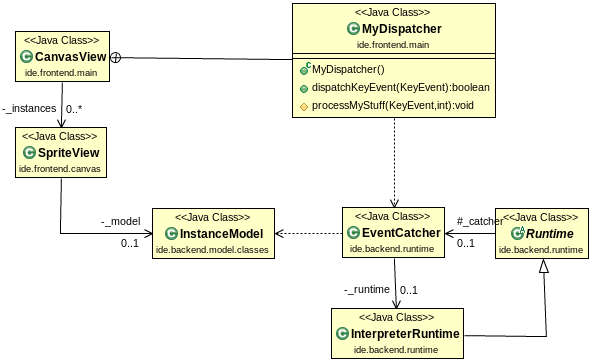
\includegraphics[scale=0.4]{AnalyseADTAlgorithm/dispatcher.png}
  \caption{EventCatcher.} 
\end{figure}

\subsection{Compileren}
\label{Compileer}
De modellen die bestaan in het programma moeten omgezet worden naar een uitvoerbaar formaat. Hiervoor is gekozen om een \textbf{Compiler} te implementeren.  \\\\
Elke visuele view van een blok heeft een model zoals uitgelegd in Sectie~\ref{Modellen}. Dit model wordt bij het compileren meegegeven aan een Compiler Klasse door de Runtime. Deze klasse is een information expert met betrekking tot compileren. De IDE gebruikt een Interface Compiler zodanig dat de gebruikte programmeertaal van de uitvoering niet direct vasthangt aan de IDE. De interface bevat verschillende functies die elk een ander type model compileren. Omdat het wireFrame ook voorgesteld wordt als een model kan het wireFrame op een gelijkaardige manier gecompileerd worden. Doordat de modellen als een boom opgebouwd zijn, kan de Compiler door deze boom lopen om een programma te compileren. Het design van de Compiler gebruikt het het visitor design patroon. Het algoritme voor het compileren van een blok wordt hiermee gescheiden van de datastructuur van de blok.\\\\
\begin{figure}[H]
  \centering
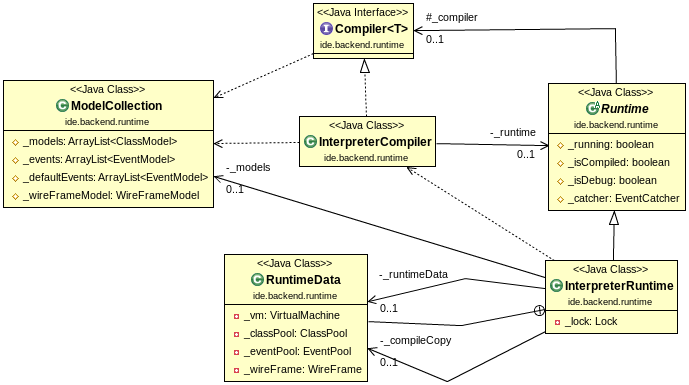
\includegraphics[scale=0.4]{AnalyseADTAlgorithm/compiler-runtime-modelCollection}
  \caption{Compiler.} 
\end{figure}

\subsubsection{Visitor patroon}
\label{visitorpatroon}
Onderstaand code fragment geeft aan hoe het visitor patroon gebruikt wordt \cite{Visitor}. De nood aan het visitor patroon komt door het feit dat Java een BlockModel niet zal downcasten naar bijvoorbeeld een PrintModel bij een functie aanroep. Hierdoor zal niet de juiste CompileBlock functie van de compiler worden aangeroepen. Door het model zelf de oproep te laten doen is dit wel mogelijk. Dit gebeurt door een compile functie van het model op te roepen en de compiler mee te geven. Het model zal nu zelf de compile functie van de compiler aanroepen waardoor de functie met juiste type parameter wordt gekozen. In dit geval PrintModel. Andere oplossingen zouden als gevolg hebben dat we de correcte functie moeten kiezen door middel van een soort switch, of dit nu via lambda functies, if-statements of een eigenlijk switch statement gebeurt. Deze oplossing is minder elegant dan het visitor patroon.

\lstset{language=Java}
\begin{lstlisting}
public class InterpeterCompiler implements Compiler<Block>{
	public Block compileBlock(PrintModel model) throws CompileException {
		if (model niet compleet) throw CompileException();
		return new PrintBlock((Block) model.getContent().compile(this));
	}
}

public class PrintModel extends BlockModel{
	public <T> T compile(Compiler<T> c) throws CompileException {
		return c.compileBlock(this);
	}
}
\end{lstlisting}

\subsection{Virtual Machine}
\label{VM}
De virtual machine zorgt voor de goede uitvoering van een enkele cycle in het programma. Er zijn verschillende gesimuleerde threads aanwezig die we processen noemen en elk van deze processen moet uitgevoerd worden. Dit is de taak van de virtual machine. Verzonden events moeten ook verwerkt worden. Er moeten nieuwe processen aangemaakt worden voor elk opgevangen event. Hiervoor is de EventDispatcher ge\"implementeerd. \\\\
De \textbf{virtual machine} bevat enkele lijsten van processen. Er is de lijst van processen die deze cycle uitgevoerd moeten worden. Een cycle wordt gedefinie\"erd als de uitvoeren van enkele stappen van deze lijst. Het aantal stappen dat van elke lijst uitgevoerd wordt, is gespecifie\"erd door de runtime, zie Sectie~\ref{debugging}. Er is een lijst van processen die de hudige stap al uitgevoerd hebben, processen die niet afgelopen zijn worden niet in deze lijst gestoken. En uiteindelijk is er een lijst waarin alle processen zitten die opgestart zijn met behulp van een verzonden event, deze lijst is chronologisch geordend. Het eerste proces in de lijst is het proces opgestart door het eerste verzonden event. Dit houdt zowel events verzonden door de GUI, als events verzonden door andere processen in. \\\\
Na het uitvoeren van een cycle, als de lijst van huidige uit te voeren processen leeg is, wordt de lijst van uitgevoerde processen samengevoegd met de lijst van processen aangemaakt door events. Een event wordt eigenlijk pas opgevangen na een cycle en dus worden alle processen opgestart door een event achteraan bijgevoegd aan de lijst van uitgevoerde processen. Deze uiteindelijke lijst zal de volgende cycle gebruikt wordt. Processen die volledig klaar zijn met uitvoeren worden verwijderd. \\\\
Als een Event verstuurd wordt zal de Virtual Machine dit Event doorgeven aan een Event Dispatcher. Dit is een Klasse die de taak voor het verzenden van Events op zich neemt. De \textbf{Event Dispatcher} kent alle verbindingen tussen de Instanties, en hiermee kunnen nieuwe processen aangemaakt worden zodat de Virtual Machine deze kan gebruiken. Deze processen worden vervolgens in de correcte lijst in de virtual machine gestoken.
\subsubsection{Een proces}
Een \textbf{proces} is een gesimuleerde thread. Deze beheert nodige data zoals een variable-stack en code. Een proces wordt uitgevoerd door de VM. Een proces kan gerunned worden en deze zal dan \'{e}\'{e}n primitieve stap \ref{primitive}uitvoeren.\\\\
Het proces bevat een stack van Blocks. Initi\"{e}l bevat die stack enkel de handler die opgeroepen is. Het bevat de instantie waarvan het de handler uitvoert. Het bevat ook een Stack van functionFrames (van Hashmaps waarbij Strings worden gemapt op Variables (zie Sectie~\ref{functionframe}).\\\\ Deze laatste stack stelt de stack van actieve functies voor. Een proces bevat een run-functie die \'{e}\'{e}n primitieve stap zal uitvoeren. Deze functie kan een event teruggeven als deze gecree\"{e}rd werd in de primitieve stap. Als het geen event terug geeft is er geen event gecree\"{e}rt maar is het proces nog niet afgelopen. Als het wel een afgelopen (de stack van Blocks is leeg) zal het een ProcesFinishedException gooien. Hierdoor weet de virtualmachine dat het event niet terug op de queue moet worden gezet. Het proces bevat ook nog een klasse ReturnVariables.\\\\ De klasse bevat ook nog een boolean locked die aangeeft als het proces verantwoordelijk is voor het locken van een variabele. Hierop kunnen er wel nog nieuwe locks gebeuren binnen dat proces. Een voorbeeld van de werking van een proces is uitgewerkt in Sectie \ref{voorbeeldvm}.

\subsubsection{FunctionFrame}
\label{functionframe}
Een functionFrame stelt het stackframe voor van een functie blok. Deze bevat een hashmap \cite{hashmap} waarbij
de lokale Variables van die functie gemapt worden op hun naam in die functie.\\\\
De keuze van een Hashmap zorgt ervoor dat het toevoegen van nieuwe variabelen en het opzoeken van bestaande in O(1) tijd kan gebeuren aangezien een functie een beperkt aantal lokale variabele bevat. Door het gebruik van een Hashmap is er ook geen extra compile stap nodig omdat we de variable dadelijk kunnen mappen op de content en geen indices van een array moeten worden berekent.\cite{hashmap}
\subsubsection{Stoppen van uitvoering}
Zoals aangehaald in Sectie~\ref{Runtime} bevat de Runtime klasse een functie die continue de VM aanroept. Als de gebruiker wenst te stoppen met uitvoering zal deze functie stoppen met uitvoeren.

\subsubsection{Functies}
\label{returnwaardes}
In de GUI zijn enkel functies ondersteund die maar \'{e}\'{e}n enkele returnwaarde hebben. De uitvoeromgeving ondersteund echter meerdere returnwaardes. Het toevoegen van meerdere returnwaardes in de IDE vereist enkel een aanpassing aan de GUI.

\subsection{Debugging}
\label{debugging}
De uitvoering moet uiteraard ook \textbf{debugging} capaciteiten bezitten. Er moest echter opgelet worden dat de structuur van de gewone uitvoering niet vervuild wordt met de toevoeging van een debugging modus. De uiteindelijke implementatie is afgeleid van de implementatie van debugging in standaard programmeertalen zoals Java of C++. Wanneer er voor deze talen gecompilleerd wordt voor debugging, word er extra data, debugsymbolen, toegevoegd aan de executable. De applicatie zal dit spiegelen en ook op bepaalde plaatsen extra debugging blokken toevoegen. \\\\
De runtime kan laten weten aan de Virtual Machine hoeveel stappen er uitgevoerd moeten worden in een cycle. Meestal zal dit aantal een stap zijn. Hierbij voert de Virtual machine een blok uit van elk proces. Voor het debuggen zal de runtime echter stellen dat de virtual machine drie blokken moet uitvoeren. \\\\
Bij de compilatie in debug-modus plaatst de compiler speciale debug blokken voor en na elke blok. Hierdoor komt het aantal op drie blokken. De eerste debug blok weet of de gecompileerde blok een breakpoint bevat. Deze zal, als er gebreaked moet worden, een break-exception gooien. Deze stopt dan de uitvoer van het programma. De uitvoer stopt voor de volledige uitvoering, elk proces zal gestopt worden. \\\\
Beide debug blokken kennen ook het model dat gecompileerd word. Als de debug blok uitgevoerd worden, zullen de blokken respectievelijk de debug-modus van het model aan of uit zetten. \\\\
Een typische uitvoering in debug-modus houdt in: zet de debug-modus van de vorige blok uit, zet de debug-modus van de huidige blok aan en ,indien er niet gebreaked is, voer de huidige blok uit. Bij het toevoegen van een proces zal de debug-modus van de handler aangezet worden. Daarna zal de eerste stap de volgende uitvoer hebben: Voer de handler uit, zet debug modus van de eerste blok aan, voer de eerste blok uit. De laatste stap van een handler zal maar een blok moeten uitvoeren, namelijk het uitzetten van de debug-modus van de handler. \\\\
Een model zal (via het observer-patroon) laten weten aan zijn views dat de debug-modus aan of uitgezet is. Deze views kunnen hier dan op reageren. Ze zullen een zwarte rand tekenen rond hun blok. Hierdoor wordt het duidelijk aan de gebruiker dat de uitvoer op deze plaats zit.

\subsection{Voorbeeld implementatie}
\label{voorbeeldvm}
Er bestaat een Klasse die een input event: event1 accepteerd. Dit event wordt afgehandeld door handler1 van de Klasse. De gebruiker heeft deze handler ge\"{i}mplementeerd in blokken op de volgende manier:
\lstset{language=Java}
\begin{lstlisting}
Event event1{
	members:
		- member1(number, value)
}
class Class1 {

	handler( event1) {
    		makeVar(number, x)
    		set(X, acces(event1, member1)
    		functieCall(functie1, parameters: x, return:x)
	}
	
	functie(functie1, parameters: z){
		while(z < 10){
		set(z, z + 1)
		}
		return z;
			
	}
	
	
}
\end{lstlisting}
Instantie instance1 is een instantie van Class1 waarnaar een instantie van event1 wordt verzonden. De eventDispatcher zal dus een proces aanmaken met instantie1 en op de Code stack de handler pushen.\\
Het uitvoeren van het proces zal in de volgende primitieve stappen gebeuren:\\\\
\textbf{Stap 1:} De handler zal zijn execute functie uivoeren. Deze zal een nieuw FunctieFrame aanmaken. Ook zal de eventInstance die mee werd gegeven bij het aanmaken van het proces op de stackframe geduwd. De blok van de handler op de Stack wordt vervangen door de inhoud.\\
\textbf{Stap 2:} De execute van makeVar zal een nieuwe variable van het type number maken op het huidige FunctieFrame.\\
\textbf{Stap 3:} De execute van Set zal de het Event in de huidige Stackframe zoeken en hieruit de juiste member halen nl. member1. De waarde hiervan wordt in x geplaatst. We gaan er van uit dat member1 $=$ 8.\\
\textbf{Stap 4:} De execute van FunctieCall doet de volgende stappen. Ophalen van de de parameter waarde die in de call staan. Deze slaat gij op in volgorde van de oproep. Hierna haalt hij het functieblok met de juiste functie naam op. Hiervan haalt hij de parameter namen op. Hij cre\"{e}ert een nieuw FunctieFrame en daarop pushed hij de parameternamen met de juiste eerder opgehaalde waarde. Hier is dit dus z met de waarde 8. Dit gebeurt achter de schermen met makeVar- en set-blokken. Hierna worden er eerst nog set-blokken voor de return waardes op de stack gepushed. Nu wordt de execute van de functie aangeroepen. Deze zal al zijn blokken op de stack pushen zonder nieuw frame te cree\"{e}ren.\\
\textbf{Stap 5:} De bovenste blok is nu de While blok. De execute van deze blok zal zijn conditie controleren nl $z < 10$ deze evalueert naar true aangezien x $=$ 8. Hierdoor zal de body van de While-blok op de code stack worden gepushed. Maar eerst wordt de While-blok er zelf ook nog op gepusht.\\
\textbf{Stap 6:} De waarde van X wordt in de set-blok verhoogt met 1.\\
\textbf{Stap 7:} herhaling stap 5.\\
\textbf{Stap 8:} herhaling stap 6.\\
\textbf{Stap 9:} De conditie van de While-blok evalueert nu naar false. Hierdoor worden er geen blokken op de code stack gepusht.\\
\textbf{Stap 10:} De return blok zoekt in de huidige FunctieFrame de waarde van z op en plaats deze in de returnVariables.\\
\textbf{Stap 11:} Aangezien de functie is afgelopen mag het FunctieFrame van de stack worden gepopt.\\
\textbf{Stap 12:} De set-blok zal nu x in het huidige FunctieFrame veranderen naar de return waarde\\
\textbf{Stap 13:} Het proces bevat geen blokken meer dus zal een ProcesFinishedException gooien naar de VM deze zal het proces verwijderen uit de queue.
 
\begin{figure}[H]
\centering
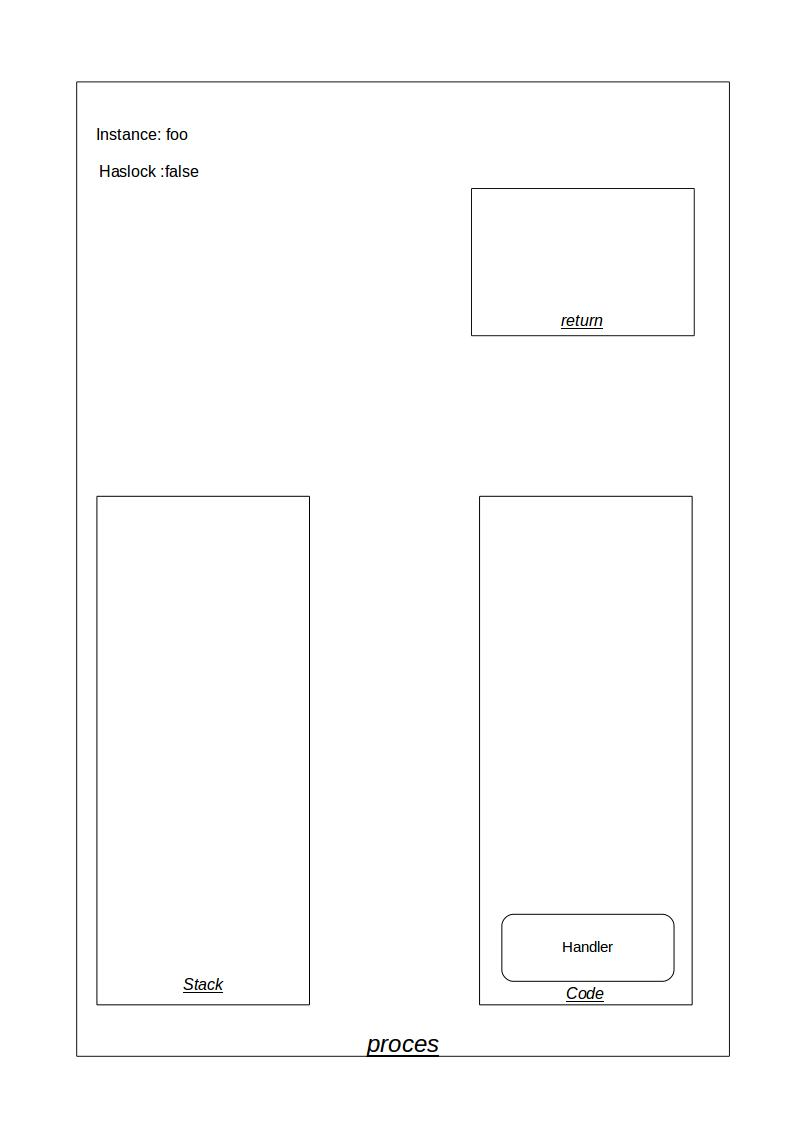
\includegraphics[scale=0.4]{AnalyseADTAlgorithm/processtappen/stap1.jpg}
\caption{Stap 1}
\end{figure}

\begin{figure}[H]
\centering
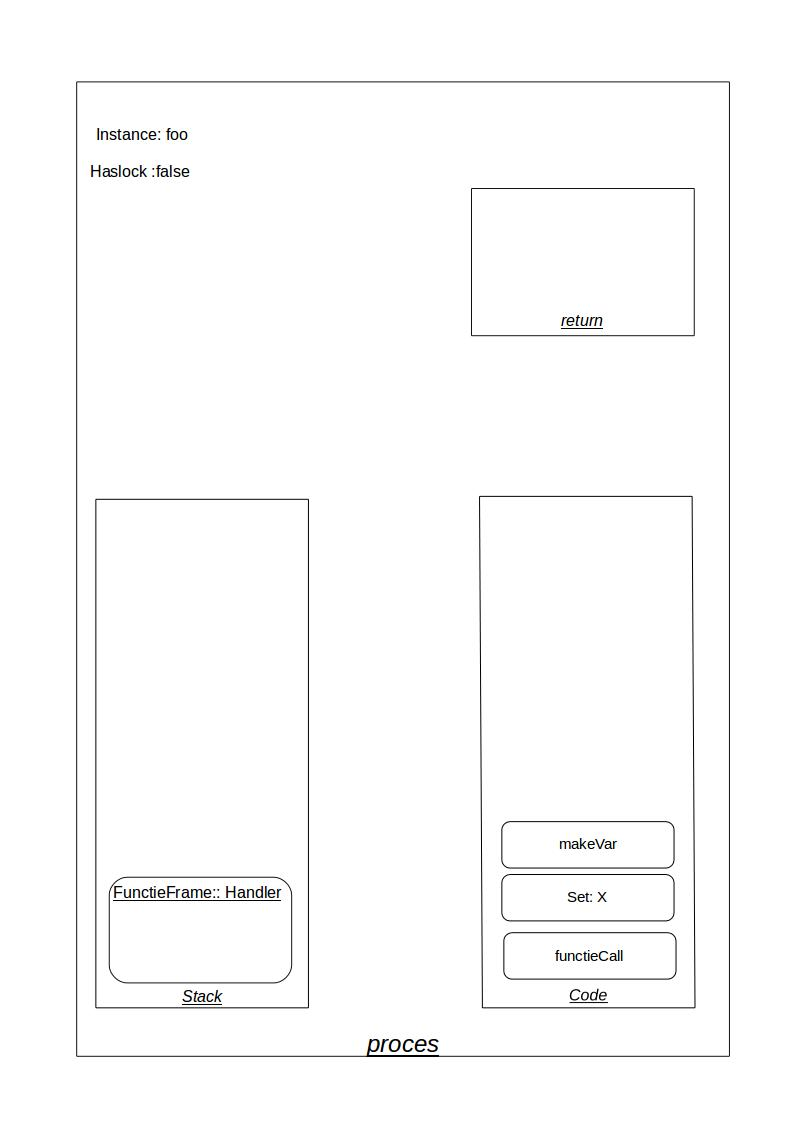
\includegraphics[scale=0.4]{AnalyseADTAlgorithm/processtappen/stap2.jpg}
\caption{Stap 2}
\end{figure}

\begin{figure}[H]
\centering
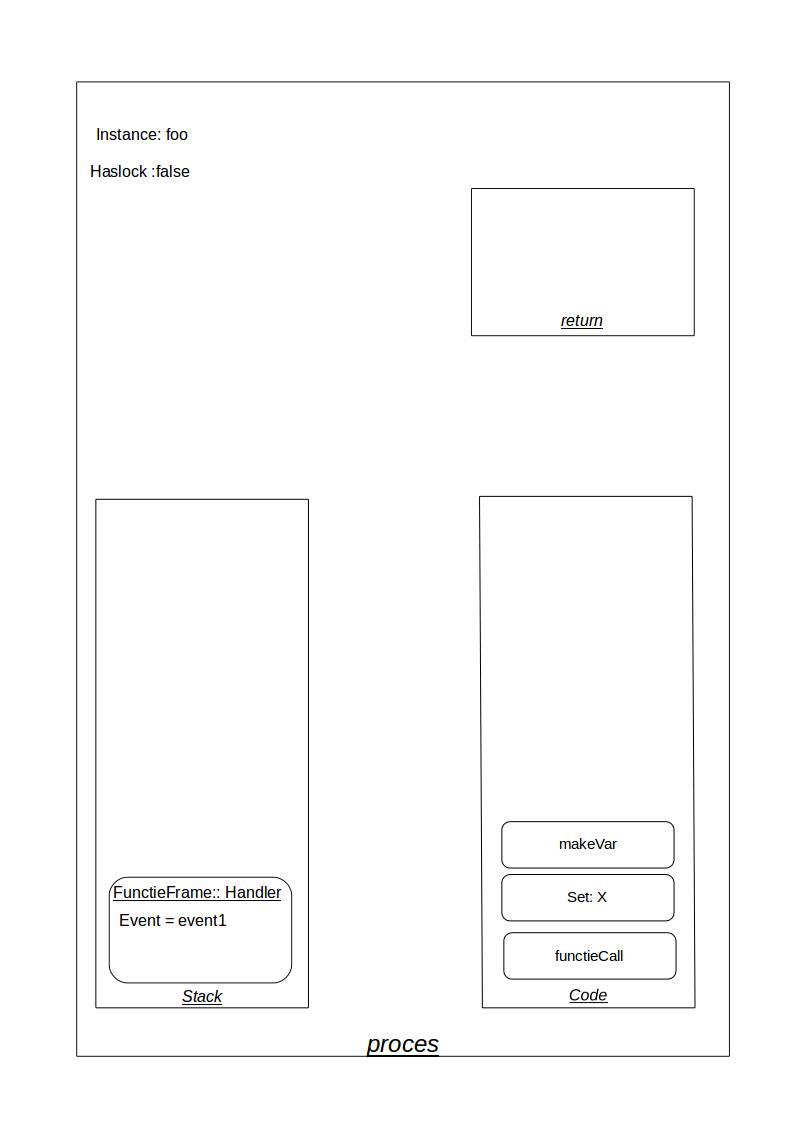
\includegraphics[scale=0.4]{AnalyseADTAlgorithm/processtappen/stap3.jpg}
\caption{Stap 3}
\end{figure}
\begin{figure}[H]
\centering
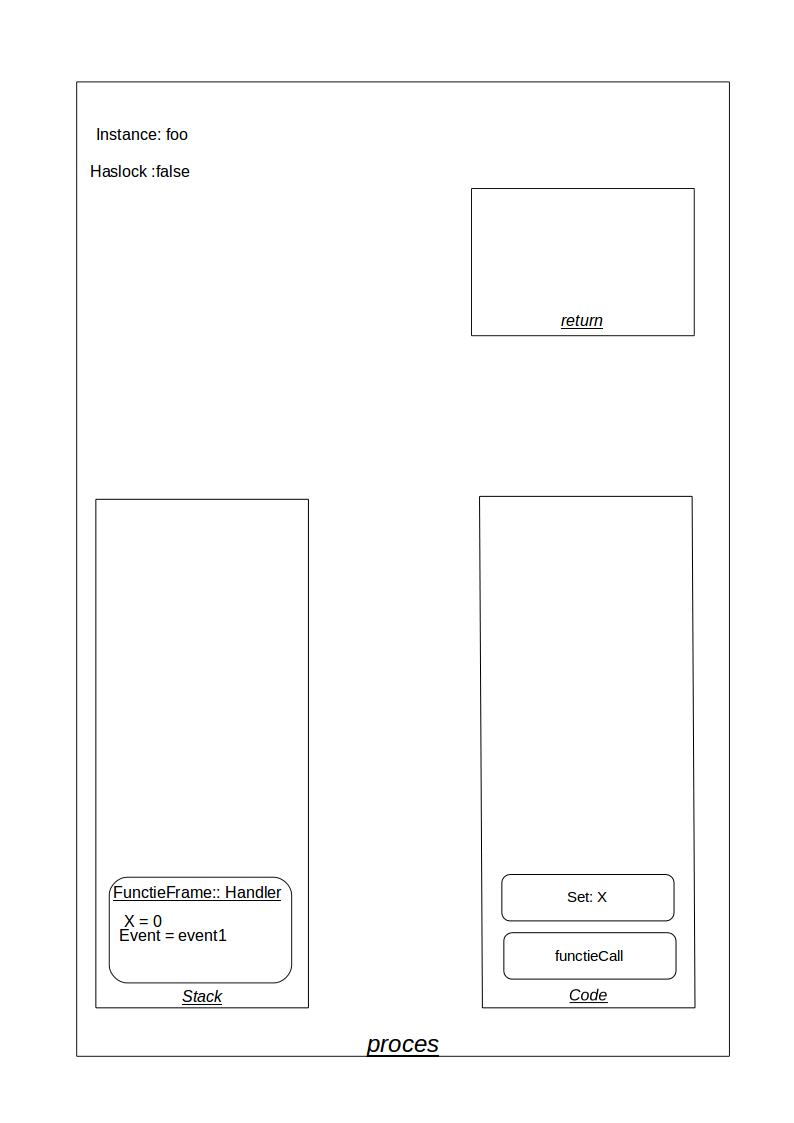
\includegraphics[scale=0.4]{AnalyseADTAlgorithm/processtappen/stap4.jpg}
\caption{Stap 4}
\end{figure}
\begin{figure}[H]
\centering
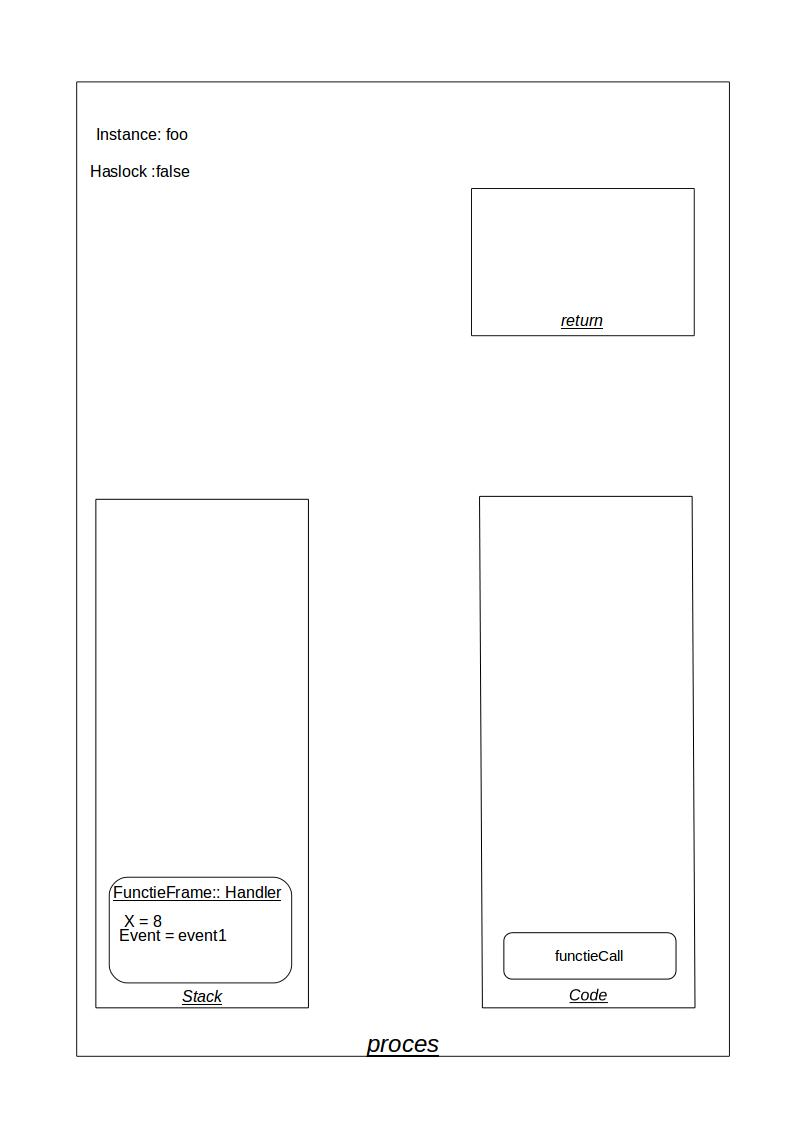
\includegraphics[scale=0.4]{AnalyseADTAlgorithm/processtappen/stap5.jpg}
\caption{Stap 5}
\end{figure}

\begin{figure}[H]
\centering
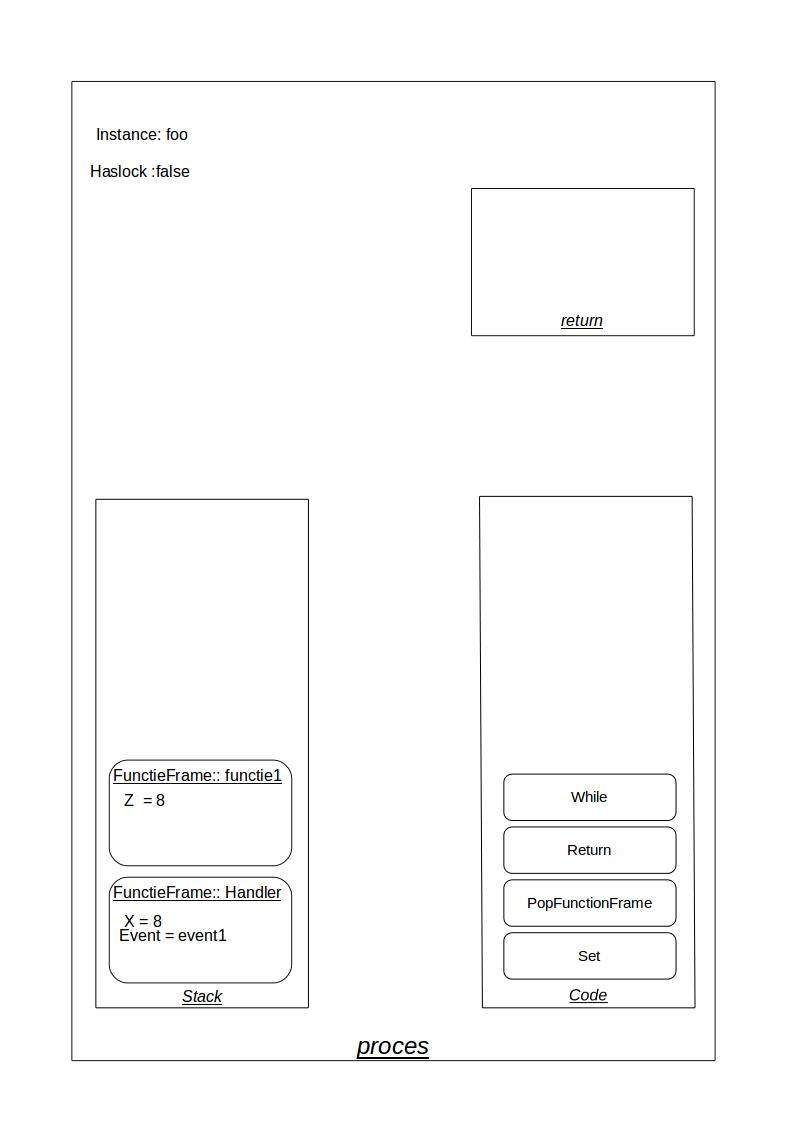
\includegraphics[scale=0.4]{AnalyseADTAlgorithm/processtappen/stap6.jpg}
\caption{Stap 6}
\end{figure}

\begin{figure}[H]
\centering
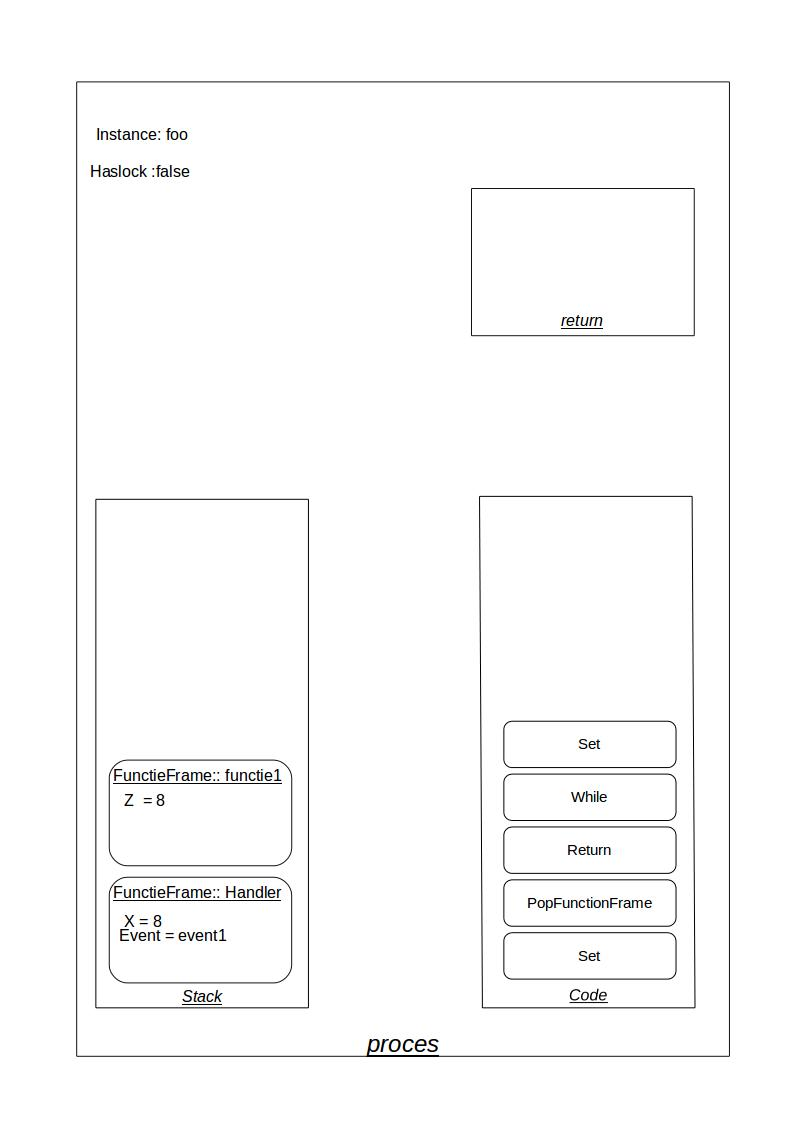
\includegraphics[scale=0.4]{AnalyseADTAlgorithm/processtappen/stap7.jpg}
\caption{Stap 9}
\end{figure}

\begin{figure}[H]
\centering
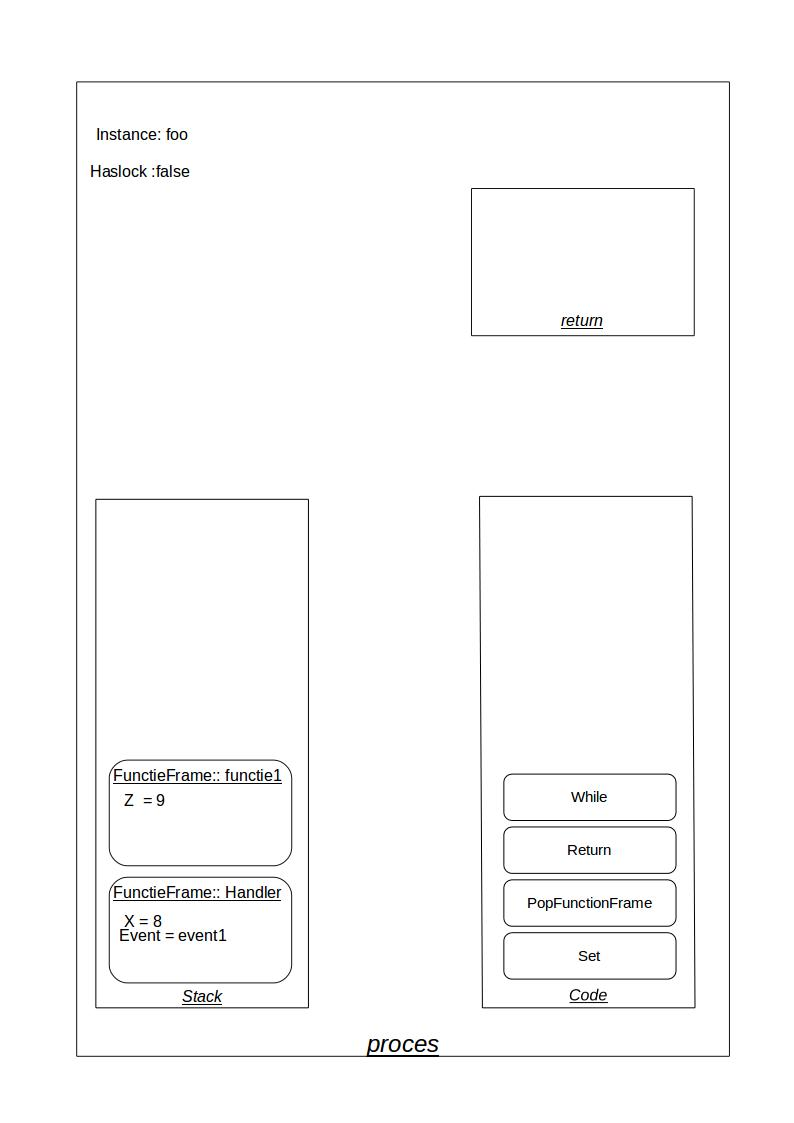
\includegraphics[scale=0.4]{AnalyseADTAlgorithm/processtappen/stap8.jpg}
\caption{Stap 10}
\end{figure}

\begin{figure}[H]
\centering
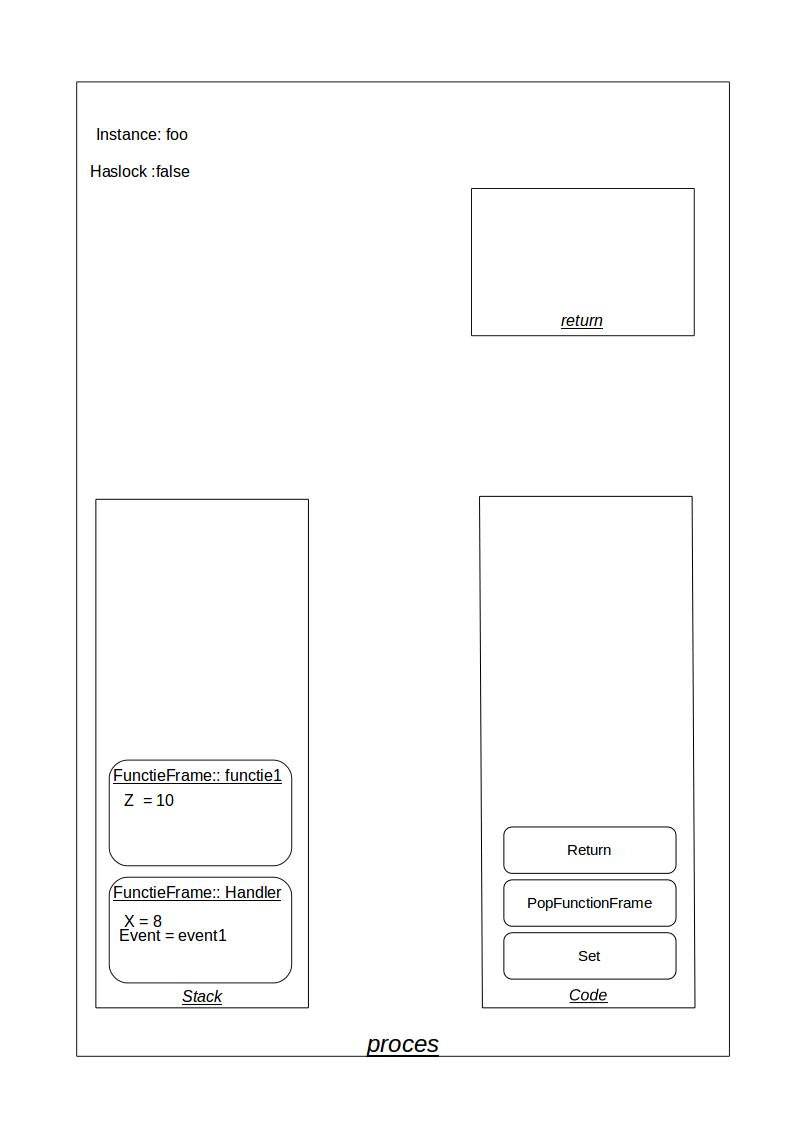
\includegraphics[scale=0.4]{AnalyseADTAlgorithm/processtappen/stap9.jpg}
\caption{Stap 11}
\end{figure}
\begin{figure}[H]
\centering
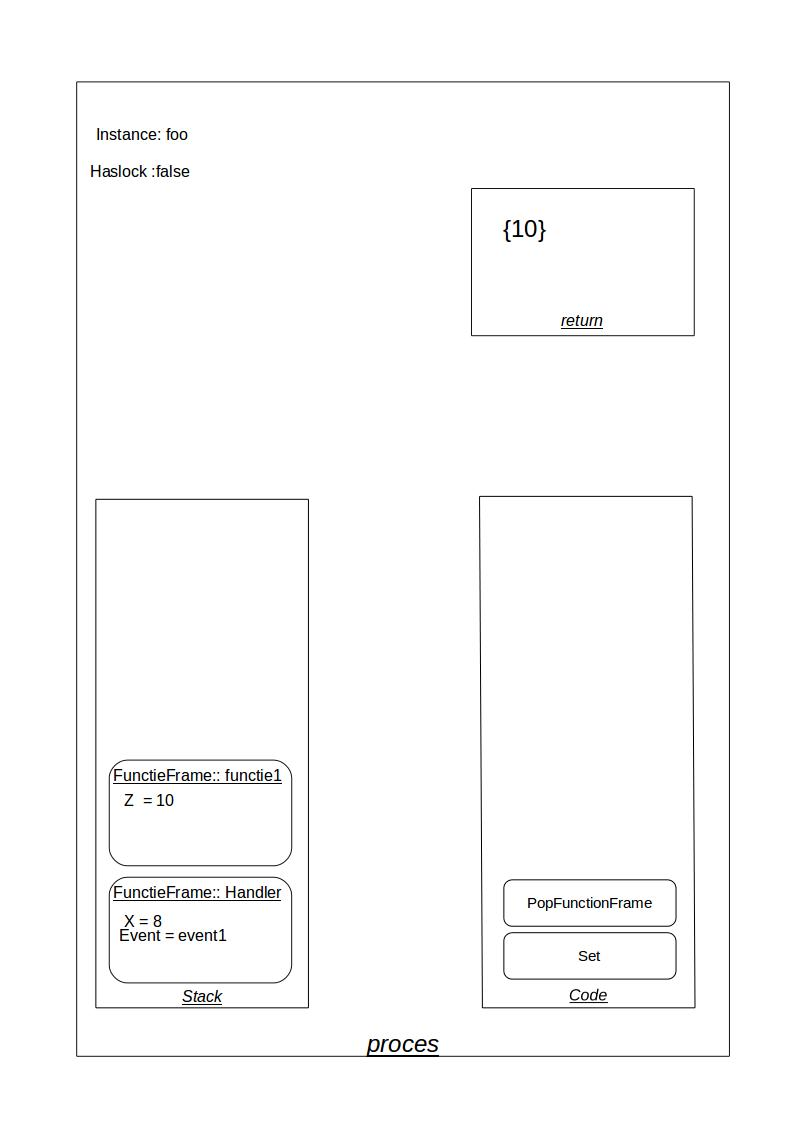
\includegraphics[scale=0.4]{AnalyseADTAlgorithm/processtappen/stap10.jpg}
\caption{Stap 12}
\end{figure}
\begin{figure}[H]
\centering
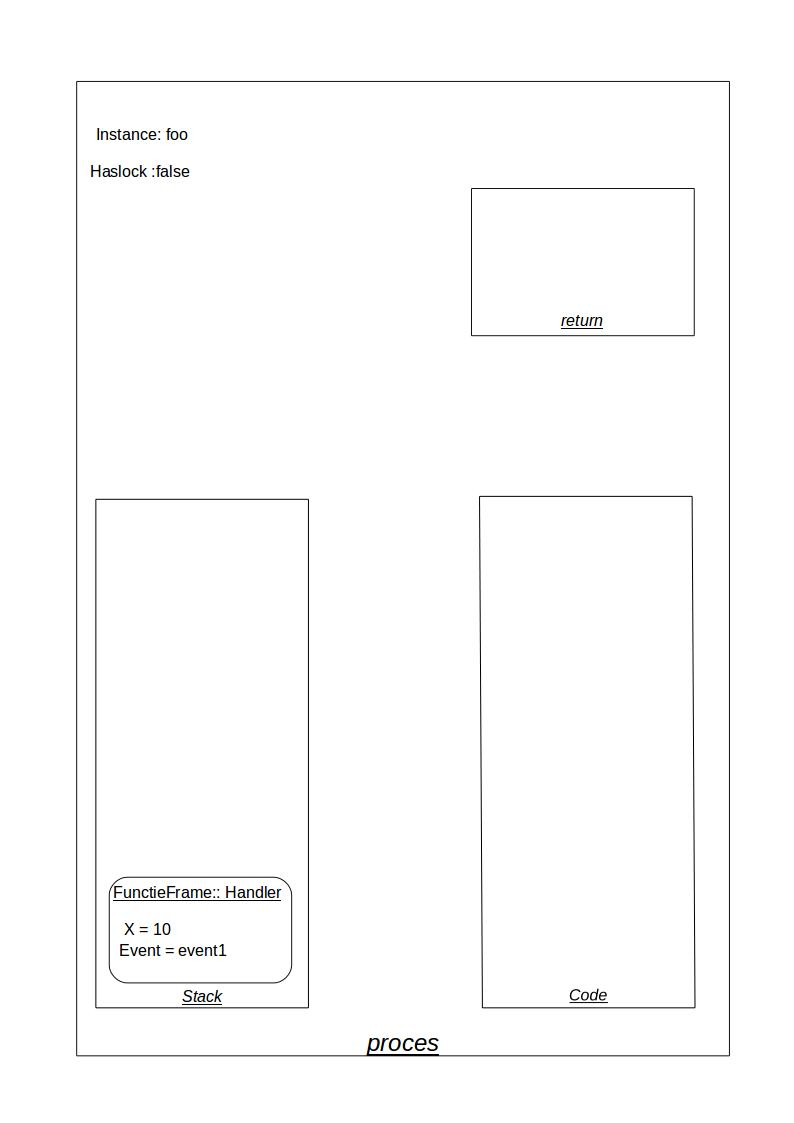
\includegraphics[scale=0.4]{AnalyseADTAlgorithm/processtappen/stap11.jpg}
\caption{Stap 13}
\end{figure}

\subsection{Lambda expressions}
\label{lambda}
Sinds 1.8 biedt Java de mogelijk aan om lambda expressies \cite{lambda} te gebruiken, we gaan hier dan ook gebruik van maken. Onze operator blok is hier geschikt voor. Via lambda expressies kan men anonieme interface methodes aanmaken. Hieronder volgt een voorbeeld waarin duidelijk volgt hoe wij het zouden gebruiken. 
\lstset{language=Java}
\begin{lstlisting}
public class Calculator {
  
    interface IntegerMath {
        int operation(int a, int b);   
    }
  
    public int operateBinary(int a, int b, IntegerMath op) {
        return op.operation(a, b);
    }
 
    public static void main(String... args) {
    
        Calculator myApp = new Calculator();
        IntegerMath addition = (a, b) -> a + b;
        IntegerMath subtraction = (a, b) -> a - b;
        System.out.println("40 + 2 = " +
            myApp.operateBinary(40, 2, addition));
        System.out.println("20 - 10 = " +
            myApp.operateBinary(20, 10, subtraction));    
    }
}
\end{lstlisting}
In de operator block zal een statische hashmap bijgehouden worden. Deze word slechts \'{e}\'{e}n keer ge\"{i}nitialiseerd. In deze hashmap worden strings gemapt op lambda functies. De string $+$ mapt op een lambda functie enz. Deze lambda functie wordt hieronder beschreven:
\begin{lstlisting}
    interface OperatorMath {
        Variable operation(Variable a, Variable b);   
    }
  
    OperatorMath addition = (a, b) -> a.addVar(b);
    OperatorMath subtraction = (a, b) -> a.subVar(b);
\end{lstlisting}

\subsection{Debugging}
\label{Debug}
De runtime kan laten weten aan de Virtual machine hoeveel stappen er uitgevoerd moeten worden in een cycle. Meestal zal dit aantal een stap zijn. Hierbij voert de Virtual machine een blok uit van elk proces. Voor het debuggen zal de runtime echter stellen dat de virtual machine drie blokken moet uitvoeren. \\\\
Bij de compilatie in debug-modus plaatst de compiler speciale debug blokken voor en na elke blok. Hierdoor komt het aantal op drie blokken. De eerste debug blok weet of de gecompileerde blok een breakpoint bevat. Deze zal, als er gebreaked moet worden, een break-exception gooien. Deze stopt dan de uitvoer van het programma. De uitvoer stopt voor de volledige uitvoering, elk proces zal gestopt worden. \\\\
Beide debug blokken kennen ook het model dat gecompileerd word. Als de debug blok uitgevoerd worden, zullen de blokken respectievelijk de debug-modus van het model aan of uit zetten. \\\\
Een typische uitvoering in debug-modus houdt in: zet de debug-modus van de vorige blok uit, zet de debug-modus van de huidige blok aan en ,indien er niet gebreaked is, voer de huidige blok uit. Bij het toevoegen van een proces zal de debug-modus van de handler aangezet worden. Daarna zal de eerste stap de volgende uitvoer hebben: Voer de handler uit, zet debug modus van de eerste blok aan, voer de eerste blok uit. De laatste stap van een handler zal maar een blok moeten uitvoeren, namelijk het uitzetten van de debug-modus van de handler. \\\\
Een model zal (via het observer-patroon) laten weten aan zijn views dat de debug-modus aan of uitgezet is. Deze views kunnen hier dan op reageren. Ze zullen een zwarte rand tekenen rond hun blok. Hierdoor wordt het duidelijk aan de gebruiker dat de uitvoer op deze plaats zit.

\section{Verschillende onderdelen van GUI}
Zoals eerder beschreven zal de GUI onderverdeeld worden in vier grote onderdelen. Namelijk ClassView, EventView, WirePanel en het Canvas. Deze structuur wordt ook door getrokken in het ontwerp van het programma. Sectie \ref{ModelCollection} bespreek de ModelCollection klasse waarin alle informatie van het programma verzameld wordt.\\\\
Uiteraard is er onderlinge communicatie nodig tussen deze verschillende onderdelen. Zo zal bijvoorbeeld het cree\"{e}ren, aanpassen of verwijderen van een klasse of Event gevolgen hebben op meerdere plaatsen in het programma.\\\\
Voor het GUI deel van het programma wordt er sterk gebruik gemaakt van het Model-View-Controlller ontwerp patroon. Hierdoor proberen we het grafische deel van het programma niet te vervuilen met applicatie logica. Voor een goede basis te hebben, zijn we vertrokken van een MVC module aangeboden uit het vak Object-geori\"{e}nteerd programmeren.\\\\
Hoewel de ModelCollection klasse alle data bevat van het programma. Hebben we ervoor gekozen om elk view een apart model tegeven. Dit omzowel de ModelCollection niet te vervuilen met View specifieke benodigdheden. Als de mogelijkheid om elke View apart te ontwikkelen. Figuur \ref{highlevelViews} toont de globale structuur van de connectie tussen de GUI en de modellen. Om de eerder vermelde gevolgen van aanpassingen door te geven in elk view. Zal elk model van een view de ModelCollection observeren voor veranderingen.\\\\
Het vervolg van deze sectie zal kort de structuur van de views bespreken. 
\begin{figure}[H]
  \centering
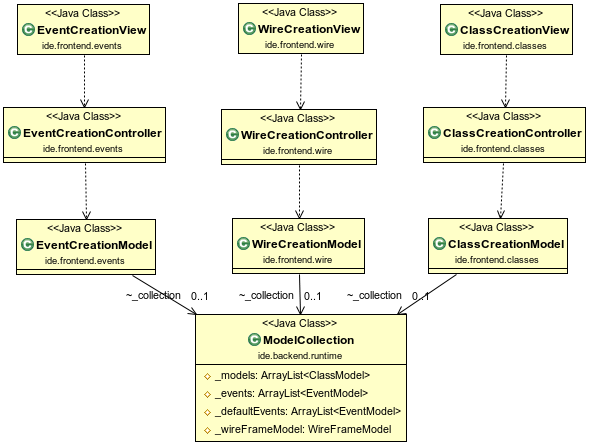
\includegraphics[scale=0.4]{AnalyseADTAlgorithm/viewsmvc/highlevel}
  \caption{Connectie model views.} \label{highlevelViews}
\end{figure}

\subsection{Klasse view}
Deze sectie bespreekt kort hoe de GUI van het klasse view is opgebouwd. Het ClassCreationView wordt gebruikt voor het aanmaken en tonen van de verschillende klassen die de gebruiker defineerd. Dit view bevat ook het paneel SelectBlocksPanel waarop de beschikbare blokken worden getoond. Dit view heeft ook de controllen over het aanmaken en plaatsen van blokken.\\\\
Het ClassCreationView bevat dus voor elke klasse een ClassView. Een Classview bestaat uit drie delen. Een paneel waarop blokken geplaatst worden. Een deel voor het inladen en selecteren van kostuums (ClassCostumeView). En tenslotte een deel voor het cree\"{e}ren en aanpassen van member variabelen (MemberVariablesView).\\\\
Het eerste deel wordt opgedeeld in twee delen. Een paneel voor de draden tussen Handlers en inputEvents en een voor de blokken. Dit wordt besproken in Sectie \ref{wires}.  Het blokken deel gebeurt door de IDEPanel-klasse. Deze bevat een dateklasse (IDEPanelData) en een klasse voor het paneel met InputEvents (ClassInputEventView). Aangezien het laatste paneel toegang moet hebben tot alle bestaande Events, kan dit via een controller naar het ClassCreationModel dewelke dan weer aan alle Events kan in de ModelCollection.
\begin{figure}[H]
  \centering 
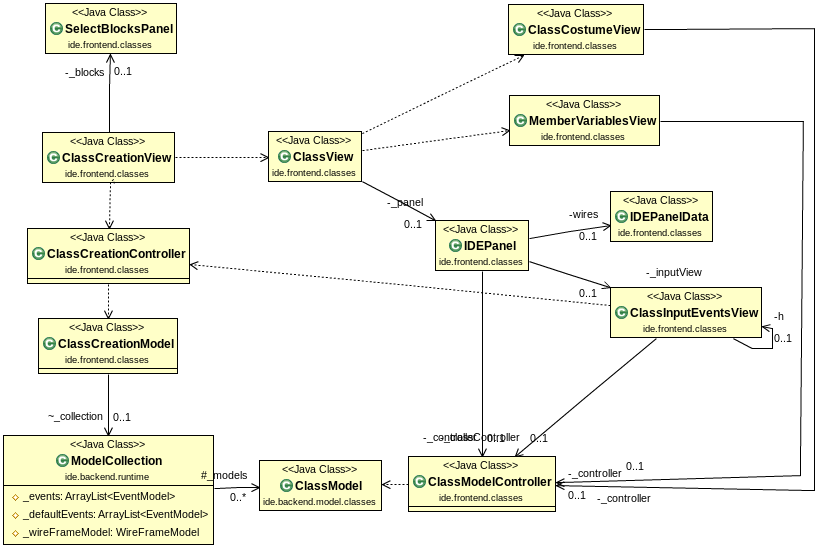
\includegraphics[scale=0.4]{AnalyseADTAlgorithm/viewsmvc/classtak}
  \caption{Klasse view tak van GUI.} \label{ClassViews}
\end{figure}

\subsection{Event View}
Deze sectie bespreekt kort hoe de GUI van het Event view is opgebouwd. Het EventCreationView wordt gebruikt voor het aanmaken en aanpassen van de verschillende Events die de gebruiker defineerd. Deze klasse bevat voor elke elk Event een EventView.\\\\
Een EventView stelt het view voor van een Event. Een EventView communiceert met zijn Model via een controller. In een EventView bevinden zich alle members van een Event. Iedere member heeft zijn EigenVariable View. Hierdoor moet bij het aanpassen van Variable enkel dit view worden aangepast.\\\\
Een variableView staat rechtstreeks in verbinding met zijn model via een controller. Hierdoor kan het type van een variable aangepast worden zonder het EventView hiermee te belasten.
\begin{figure}[H]
  \centering 
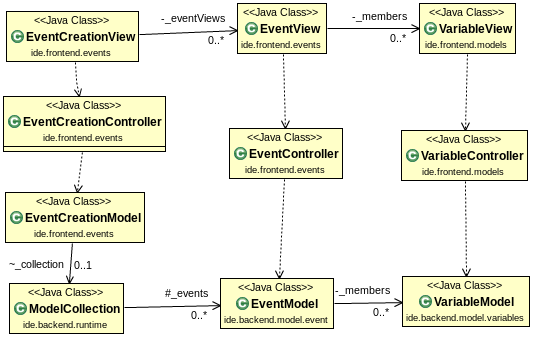
\includegraphics[scale=0.4]{AnalyseADTAlgorithm/viewsmvc/EventTak}
  \caption{Event view tak van GUI.} \label{EventViews}
\end{figure}

\subsection{Wire View}
\label{filter-view}
Deze sectie bespreekt kort hoe de GUI van het Wire view is opgebouwd. Het WireCreationView bestaat uit drie delen:
SelectInstancePanel, WirePanel en EventFilterPanel. SelectInstancePanel staat in voor de creatie van nieuwe instanties. WirePanel wordt gebruik voor het maken van connecties tussen instanties.\\\\
Aangezien Wires worden getekend op de manier zoals beschreven in sectie \ref{wires} is er geen nood voor een aparteView voor elke Wire. Voor het tekenen van de Wires wordt er gebuik gemaakt van de Input- en Output Event knoppen op een instanceView. Het toevoegen van een Wire gebeurt via de WireCreationController.\\\\
EventFilterPanel regelt welke Wires er moeten getekend worden op het WirePanel.
\begin{figure}[H]
  \centering 
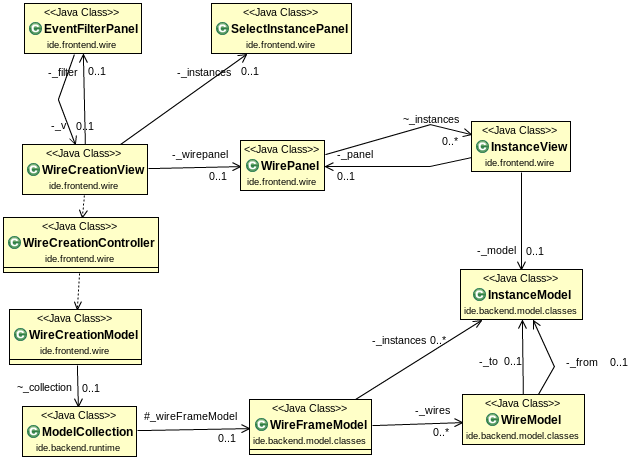
\includegraphics[scale=0.4]{AnalyseADTAlgorithm/viewsmvc/wiretak}
  \caption{Event view tak van GUI.} \label{WireViews}
\end{figure}

\subsection{Drag and drop}
\label{dnd}
Het tekenen van blokken en het drag en drop systeem hebben we zelf ge\"implementeerd. De reden om een eigen drag-and drop systeem te implementeren vindt u in secite \ref{dndProbleem}. De custom drag-and drop maakt gebruik van AWT Shapes en van Swing JComponents. \\\\
Voor de drag-and drop zijn enkel de meest externe blokken gekend. Door een simpele berekening (kijken of de muis zich binden een externe blok zit) kan de blok gevonden worden waarover de gebruiker hovert. Zodra het systeem identificeert over welke externe blok de gebruiker een blok loslaat, kan het er berekent worden waar in de hi\"erarchie de losgelaten blok geplaatst moet worden. \\\\
Een blok kent zijn specifieke regels. Hij kan zeggen of hij een blok kan bevatten, of een andere blok mogelijks genest kan worden, en hij kan dit opvragen aan zijn kind-blokken indien hij deze heeft. De meeste externe blok vraagt de meest geneste blok aan die de losgelaten blok kan bevatten. \\\\
Hierna wordt bepaald welke visuele veranderen er moeten optreden, zoals het verhogen van zijn hoogte. Een blok kan de hoogtes en breedtes van zijn kindblokken opvragen. \\\\
Omdat enkel de meest externe blokken gekend zijn aan het drag-and drop systeem moeten alle JComponents gebonden zijn aan de externe blokken. Een blok kan aan zijn kinderen zijn JComponents (en hun locaties relatief aan hun eigenlijke parent-blok). Deze berekent nieuwe locaties en kan deze aan zijn parent geven als deze bestaat, of de JComponents binden aan zichzelf zodat ze zichtbaar worden op het scherm.
\subsection{Wires}
In de IDE wordt er zowel voor het verbinden van Events tussen instances in het WireFrame als voor verbinden van Input Events en Handlers in ClassView gebruik gemaakt van wires die automatische worden getekend. Voor het tekenen wordt er gebruik gemaak van \texttt{QuadCurve2D} \cite{QuadCurve}. Wires worden altijd op de voorgrond getekend door gebruik te maken van een \texttt{JLayeredPane} \cite{LayedPane}. Deze bestaat steeds uit twee panels namelijk een panel voor de wires en een voor de eigenlijke blokken. Het eerste wordt louter gebruikt voor het tekenen van de Wires en zal geen input events van de gebruiker opvangen.\\\\
Als er een linker muis klik wordt geregistreed op het panel van de blokken zal er berekend worden als er op een wire wordt geklikt. Als dit het geval is zal de eerste Wire die de klik bevat als geselecteerde Wire worden genomen.\\\\
Bij het bewegen van het panel waarop de blokken zich bevinden of het bewegen van de blokken zelf zal ervoor zorgen dat alle wires opnieuw moeten worden berekend en opnieuw moeten worden getekend.

\begin{figure}[H]
  \centering
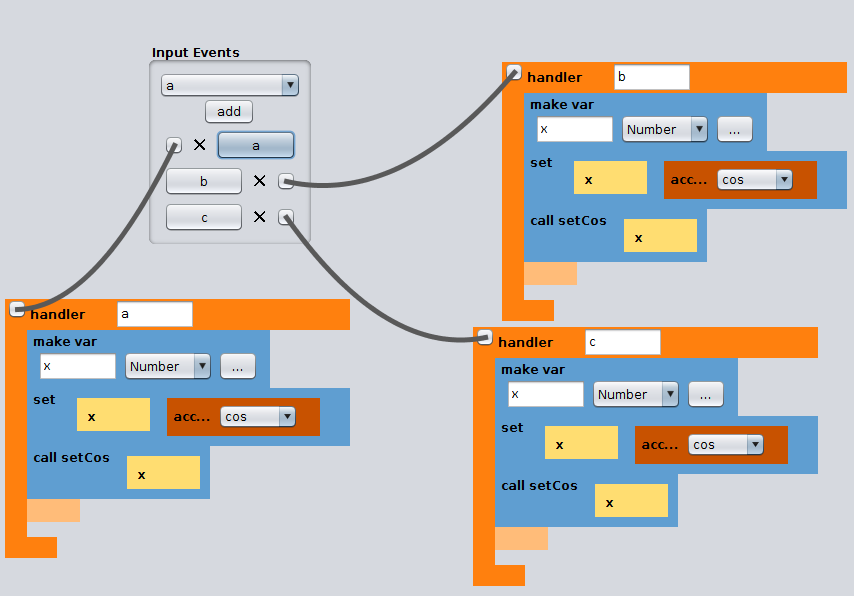
\includegraphics[scale=0.4]{AnalyseADTAlgorithm/wires.png}
  \caption{Wires.} \label{wires}
\end{figure}
\begin{figure}[H]
  \centering
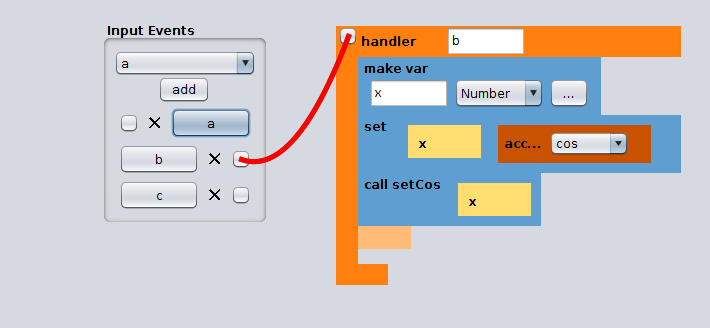
\includegraphics[scale=0.5]{AnalyseADTAlgorithm/wireSelected.png}
  \caption{Wire selected.} \label{wireSelected}
\end{figure}

\end{document}